\documentclass[conference]{IEEEtran}
\usepackage{url}
\usepackage{algorithm}
\usepackage{algorithmic}
\usepackage{epsfig}
\usepackage{minted}
% \usepackage[total={6.5in,9in}, top=1.25in,left=0.9in]{geometry}
%\usepackage[text={6.5in,9in},centerpage,includefoot]{geometry}
% \usepackage{setspace}
\usepackage{color}
\usepackage{url}
\usepackage{balance}

\definecolor{grey}{RGB}{200,200,200}
\newcommand{\hilite}[1]{\colorbox{grey}{#1}}
\newcommand{\hilitey}[1]{\colorbox{yellow}{#1}}
\newcommand{\hiliting}[1]{\colorbox{grey}{#1}}
\newcommand{\INDSTATE}[1][1]{\STATE\hspace{#1\algorithmicindent}}
\long\def\todo#1{\hilitey{{\bf TODO:} {\em #1}}}
\long\def\shorten#1{}
\def\azdb{\hbox{\sc AZDBLab}}
%\def\azdb{\hbox{\sc DBLab}}
\def\QatC{Q{@}C}
\long\def\comment#1{}
%c2j: Conference to Journal: first parameter is conference, second is journal
% For Conferences: c2j#1#2{#1}
% For Journals: c2j#1#2{2}
\long\def\c2j#1#2{#1}

\begin{document}
%don't want date printed
\date{}

%make title bold and 14 pt font (Latex default is non-bold, 16 pt)
\title{{\sc AZDBLab} : A Laboratory Information System for Empirical Studies on DBMSes}
%
\author{
DRAFT
%\IEEEauthorblockN{Young-Kyoon Suh, Richard T. Snodgrass}
%\IEEEauthorblockA{{\it Dept. of Computer Science}\\
%{\it University of Arizona}\\
%{\it Tucson, Arizona, USA, 85721}\\
%{\tt \{yksuh, rts\}@cs.arizona.edu}}
}

\maketitle

\begin{abstract} 
%Understanding a variety of behaviors present in DBMSes 
%can give an importance implication database query optimizers to improve. 
%There has been no system to study these aspects across different DBMSes. 
%This scientific approach leads to fundamental improvements 
%of database query optimizers. 
%To address this ,
%There has been no system of allowing database researchers to 
%simultaneously run experiments on different DBMSes and seamlessly analyze the results, 
%to better understand a variety of behaviours of database query optimizers. 
In database field, scientific approach has been much less prominent while very stong 
mathematical and engineering work has been done. 
Understanding database query optimizers is of critical importance in a sense that it can provide 
great insights into their improvements by looming which parts should be reexamined. 
However, there has been no system for supporting this scientific approach in which one can 
simultaneously run and monitor a variety of experiments on DBMSes and analyze the 
results to test his/her hypotheses. 
In this paper, we introduce a novel laboratory information system, 
called {\em Arizona Database Laboratory} ({\sc AZDBLab}), of allowing database researchers 
to empirically study DBMSes. 
%
%Understanding database query optimizers is of critical importance in a sense that it can provide 
%great insights into what parts of the optimizers should be examined for their improvements. 
%However, this scientific approach has been much less prominent in database field while very stong 
%mathematical and engineering work has been done. 
%For instance, there has been no system of allowing database researchers to 
%simultaneously run experiments on different DBMSes and seamlessly analyze the results. 
%To support this scientific, empirical study on DBMSes, in this paper we introduce a novel laboratory information system, 
%called {\em Arizona Database Laboratory} ({\sc AZDBLab}). 
\end{abstract}

% A category with the (minimum) three required fields
%\category{H.4}{Information Systems Applications}{Miscellaneous}
%A category including the fourth, optional field follows...
%\category{D.2.8}{Software Engineering}{Metrics}[complexity measures, performance measures]

\section{Introduction}\label{sec:intro}
%Understanding database query optimizers is of critical importance in a sense that it can provide 
%great insights into what parts of the optimizers should be examined for their improvements. 
%Also, it can ultimately derive predictive theories about how optimizers as a general class behave, which will be very 
%useful in the enhanced design of query optimizers. 
%Despite these strengths, this scientific approach has been much less prominent in database field while very stong 
%mathematical and engineering work has been done. 
%For instance, there has been no system of allowing database researchers to 
%simultaneously run experiments on different DBMSes and seamlessly analyze the results. 
%To support this scientific, empirical study on DBMSes, we introduce a novel laboratory information system, 
%called {\em Arizona Database Laboratory} ({\sc AZDBLab}). 
In database field, scientific approach has been much less prominent while very stong 
mathematical and engineering work has been done. 
Understanding database query optimizers is of critical importance in a sense that it can provide 
great insights into their improvements by looming which parts should be reexamined. 
Also, it can ultimately derive predictive theories about the database optimizer behavior, thereby leading to their 
enhanced design. 
However, there has been no system for supporting this scientific approach in which one can 
simultaneously run and monitor a variety of experiments on DBMSes and analyze the 
results to test his/her hypotheses. 
In this paper, we introduce a novel laboratory information system, 
called {\em Arizona Database Laboratory} ({\sc AZDBLab}), of 
allowing database researchers to empirically study DBMSes. 

{\sc AZDBLab} consists of 45K source lines of code, and currently supports experiments on five DBMSes, 
three commercial and two open-source. 
 {\sc AZDBLab} is effectively an electronic laboratory notebook. 
Within this environment, one can design and specify experiments, 
schedule these experiments, monitor them when they are running, 
record both independent variables (those controlled by the experimenter) and 
dependent variables (those resulting from the experiment), and do analyses on the data. 
{\sc AZDBLab} runs on a hardware lab of dedicated machines, 
one each for each subject DBMS and one to host the DBMS that stores the lab notebooks, called {\em labshelves}. 
Having dedicated hardware allows us to worry less about other processes running on the machines 
that could dirty the results (these machines are only for experiments), and allows us to run extensive 
experiments taking days or weeks. 

The key contributions of this paper are as follows.
\begin{itemize}
\item We introduce a novel {\em laboratory information system}, called {\em Arizona Database Laboratory} ({\sc AZDBLab}), 
for supporting empirical studies on a variety of DBMSes. 

\item We present various {\em plugin}s enriching the extensibility of {\sc AZDBLab}. 

\item We propose a {\em robust} methodology of running an experiment in {\sc AZDBLab}. 

\item We present the automated result analysis process incorporated into {\sc AZDBLab}. 

\end{itemize}

\section{Motivation}\label{sec:motivation} 
There are questions concerning fundamental limits of database management system (DBMS) 
architectures that simply cannot be answered by investigating a single algorithm or even a single DBMS. 
Rather, addressing such questions requires the development of {\em predictive models across multiple DBMSes}. 

The objective is to understand database management systems as a {\em general} class of computational artifacts, 
to come up with insights and ultimately with predictive models about how such systems, again, as a 
general class, behave, by studying multiple DBMSes at a time. 
These models are articulated and thoroughly tested, in order to 
understand more deeply the behavior of query optimization and evaluation across multiple DBMSes. 
They can be eventually used to improve DBMSes through engineering efforts 
that benefit from the fundamental understanding that this perspective can provide. 

$\azdb$ has been designed and developed over seven years, to help us 
reach this overarching goal - to {\em predict important characteristics} of DBMSes to determine {\em fundamental limits}.  
$\azdb$ allows us to perform experiments for quantitatively studying these fundamental questions concerning 
many of the components\footnote{These cover (i) {\em cardinality estimation} (identifying what affects the accuracy of cardinality estimates), 
(ii) {\em operator impact} (characterizing how specific types of operators - e.g., {\em joins}, {\em projection}, 
{\em sorting} affect the accuracy of cardinality estimates, execution time estimates, and optimal plan selection),
(iii) execution plan search space (determining its detailed inner structure)} of a DBMS. 
As an experiment tool, $\azdb$ coordinates the running, data collection and analysis of such experiments. 
It will also be broadened to support experiment replication, provenance maintenance, a more variety of experiment 
scenarios (to be discussed), and more experiment subjects (equivalent to DBMSes). 
Thanks to this research infrastructure by $\azdb$, our empirical study on DBMSes 
has already yielded structural models that identifies across two commercial and two open source DBMSes 
some of the causes of varying query time measures\cite{Currim} and suboptimality (when the DBMS chooses a wrong plan).

In the next section, we will present the overall architectural components of $\azdb$. 

%The scope of this investigation will be significantly broadened to consider many of the components of
%a modern DBMS, including (i) cardinality estimation (identifying what affects the accuracy of 
%cardinality estimates), (ii) operator impact (characterizing how specific types of operators-e.g., joins, projection, 
%sorting—affect the accuracy of cardinality estimates, execution time estimates, and optimal plan selection), 
%(iii) execution plan search space (determining its detailed inner structure), and (iv) transaction and 
%concurrency control (specifying how throughput and disk utilization depend on multiprogramming level, how the 
%presence of hot spots affect this interaction, and when thrashing occurs). 

\section{Architecture}\label{sec:architecture}
As shown in Figure~\ref{fig:azdblab_arch}, $\azdb$ consists of {\em labshelves}, 
{\em executor},  {\em observer} and {\em plugins}. 
We describe each of the components of $\azdb$ in the next sections. 

\begin{figure}[t]
\centering
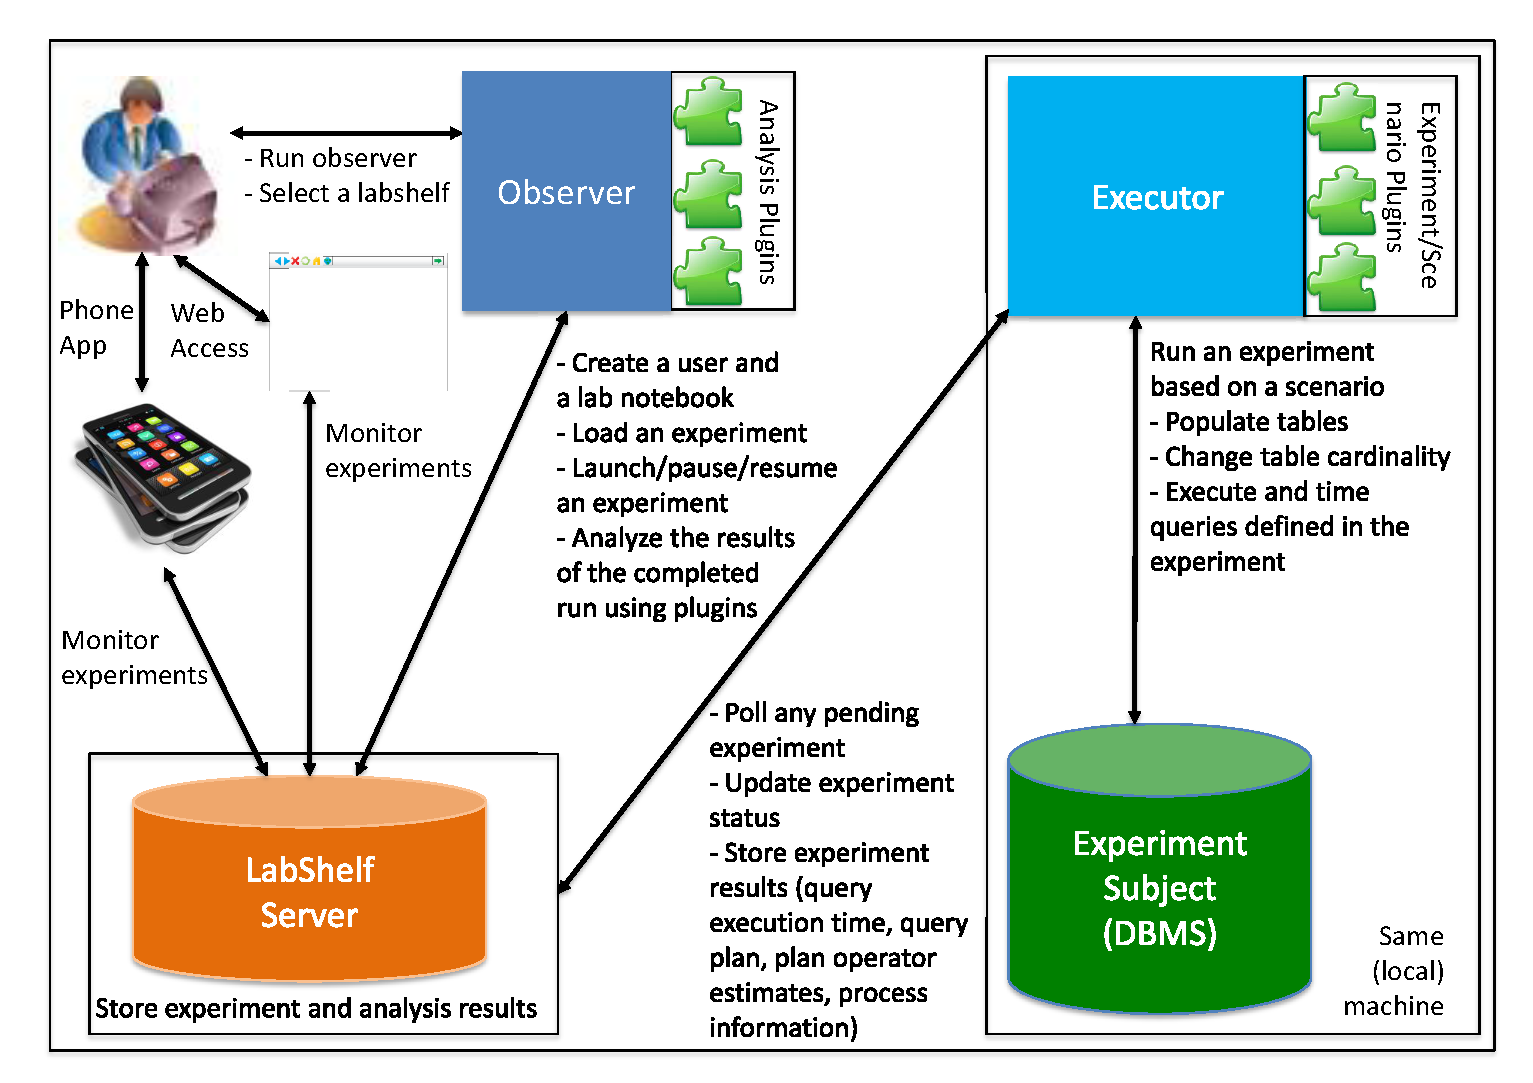
\includegraphics[scale=0.4]{./figures/azdblab_arch}
\caption{{\sc AZDBLab} archiecture~\label{fig:azdblab_arch}}
\end{figure}

\subsection{LabShelves}
A labshelf abstracts experimental data. It retains a versioned-schema 
and complies with the {\em 7-W model}~\cite{Ram}. 
Namely, the schema for a labshelf captures {\em who}, {\em what}, {\em when}, {\em which}, {\em where}, 
{\em why}, and {\em how}. It is a fully append-only database~\cite{Snodgrass99}. 
That said, there is provenance 
that the system does not yet capture. The schema also evolves as we need to capture more data for our study. 
The labshelf data are stored and managed by a dedicated server, 
running separated from other $\azdb$ components. 

\begin{figure*}[htp!]
\centering
\includegraphics[scale=0.33]{./figures/observer_gui}
\caption{{\sc AZDBLab} observer\label{fig:observer_gui}}
\end{figure*}

\subsection{Executor}
Executor is the $\azdb$ component that executes experiment queries 
and stores the query execution results into a labshelf. 
To avoid undesirable latency by network traffic, we ensure that the executor must be running 
on the same machine running a DBMS as an experiment subject. 

\subsection{Observer}
Observer is the $\azdb$ component that provides a login user 
with GUI necessary to run an experiment and analyze the experiment results. 
When launching observer, the login user is asked to choose a labshelf. 
Observer then loads data from the chosen labshelf and expose them to 
the login user if any. The data, which can be also created by the login user, 
includes a labshelf user(s), a notebook(s), an experiment(s), 
an experiment run(s), and query execution results in the experiment run(s). 

Figure~\ref{fig:observer_gui} illustrates the GUI screenshot of observer. 
The following nodes in the LHS of the GU are organized in a tree-structured way 
(although the list is flattened due to too deep nesting). 

\begin{itemize}
	\item User Node 

	\item Notebook Node

	\item Scenario Node

	\item Experiment Node 

	\item Data Definition Node

	\item Query Generation Definition Node

	\item Completed Run Node 

	\item Query Node

	\item Plan Node

	\item Papers Node
	
	\item Analysis Node
		
	\item Analytic Specification Node

	\item Aspect Specification Node

	\item Defined Queries Node	

	\item Aspect Definitions Node

	\item Analytic Definitions Node

	\item Pending Run Node

	\item Running Run Node

	\item Paused Run Node

	\item Aborted Run Node

	\item Plugin Node 

	\item Executor Node

\end{itemize}

\subsubsection{Decentralized Architecture}
Discuss the decentralized architecture of {\sc AZDBLab}. 
(Ben may describe this section.)

\begin{itemize}

\item Web Application 

\item Phone Application
\end{itemize} 

%% Describe the role of observer
%Observer provides a login user with GUI to run an experiment. 
%When launching observer, the login user is asked to select a labshelf. 
%Then, observer loads data stored in the chosen labshelf. 
%The data includes a labshelf user(s), a notebook(s), an experiment(s), an 
%experiment run(s), and query execution results in the experiment run(s). 
%The login user can also create a 

\subsection{Plugins}
The most outstanding feature of {\sc AZDBLab} is its 
unlimited extensibility by a variety of plugins. 
In this section, we discuss how a plugin is loaded into {\sc AZDBLab} 
and present different types of plugins and their roles. 

\subsubsection{Plugin Management}

Each plugin is developed as a {\em .jar} file. 
It is put into {\em plugins} subdirectory. 
When observer is launched, {\em master plugin manager} 
examines each plugin class in the plugin sub-directory 
where {\sc AZDBLab} is located.  Also, 
the manager classifies the identified along with 
its type to be discussed in the next section. 
%By preserving independence of the experiment
%% Describe a variety of plugins

\subsubsection{Plugin Type}

\begin{itemize}

\item Experiment Subject : {\sc AZDBLab} treats a DBMS as {\em experiment subject}. 

\item Scenario : A {\em scenario} defines an experiment scenario. 
It has two kinds of subclasses as follows.

\begin{itemize}
\item {\em ScenarioBasedOnCardinality} defines a scenario taking each table cardinality as a unit of task 
\item {\em ScenarioBasedOnQuery} defines a scenario taking each query as a unit of task 
\end{itemize}

\item Evaluation : $\azdb$ provides {\em evaluation plugins} for analyzing query execution results. 
Currently, there are two types of evaluation plugins in $\azdb$. 

\begin{itemize}
\item Query Stat (Evaluation) plugin parses the process information string (provided by Process Analyzer) and 
populates the per-query execution table and per-process (within the same query execution) information tables. 
The per-query execution table stores numbers of phantom/started/stopped processes, number of faults, and 
overall user/low priority/system mode, idle task, IO wait, and IRQ, Soft IRQ, and steal and stolen ticks. 

%(\item Sanity Check (Evaluation) plugin performs sanity checks on completed query executions 
%and populates the violation results. The sanity checks include number of queries not executed, 
%excess
%)

\item Process Information (Evaluation) plugin extracts 
the name and frequency of processes observed at a completed run or at a notebook. 
This process information is referenced by Process Analyzer, which will be discussed soon, 
so that the most frequently executed processes will be checked first for minimizing 
increasing their ticks during process examination.  

\end{itemize}

\end{itemize}

\subsubsection{Versioning}
Refer to {\sc AZDBLab} guides. 

\subsection{Utilities}
In this section, we introduce a few utilities in $\azdb$. 

\subsubsection{{\sc AZDBLab} Labshelf Creator}
Literally, {\sc AZDBLab} Labshelf Creator is responsible for creating all the tables under a specific labshelf version 
of {\sc AZDBLab}. It asks and encrypts labshelf name, password and JDBC connection string 
and then creates an XML file having the input data and lastly saves the XML file as a {\em plugin} in the {\em plugins} directory. 

\subsubsection{Process Analyzer}
Process analyzer provides the information of all the processes running around query execution. 
Specifically, it compares running-process snapshots before and after query execution and 
records the difference into a {\em string} along with a query execution result. 
\todo{Refer to metrology paper.}

\subsubsection{Logger}
$\azdb$ logger extends {\tt Logger} of {\tt log4j}.  
As other loggers, its primary purpose is to record into a file important running events of observer or executor 
and to check what was happening when they got hung or killed. 	 

\subsubsection{Watcher}
$\azdb$ watcher is designed to be immediately notified of when something bad happens while executor runs an experiment. 
\todo{Jen can write this subsection.}

\section{Running Experiments}\label{sec:running_exp} 
In this section, we describe how an experiment is written and run in $\azdb$. 
Figure~\ref{fig:exp_proc} depicts the overall experiment procedure in $\azdb$.  
An $\azdb$ user first needs to write his/her own (experiment) {\em scenario}. 
Along with the scenario, he should define how data should be populated 
(data population spec), how table cardinalities should vary (table cardinality variation spec), 
and how queries are generated (query generation spec). 
By collecting these specs, an experiment spec can be written. 
In turn, the experiment can be loaded and run through observer. Once the experiment is 
complete, he can analyze the experiment results. 

\begin{figure}[t]
%\begin{tabbing}
%\quad\quad\=\quad\quad\=\quad\quad\=\quad\quad\=\quad\quad\=\quad\quad\=
%\quad\quad\=\quad\quad\=\quad\quad\=\quad\quad\=\quad\quad\=\quad\quad\=\quad\quad\kill
\begin{center}
\begin{algorithmic}
{\bf Algorithm} $runExperiment$($labUser$, $labNoteBook$, $expName$, $dbms$) : \\
	\STATE $experiment$ $\leftarrow$ $getExperiment$($labUser$, $labNoteBook$, $expName$)\\
    \STATE $expRun$ $\leftarrow$ $getExperimentRun$($experiment$)\\
    \STATE $expSubject$ $\leftarrow$ $expRun$.$getExperimentSubject$($dbms$) \\
    \STATE $expSubject$.$dropAllInstalledTables$()\\
    \STATE $scenario$ $\leftarrow$ $expRun$.$getScenario$()\\ 
    \STATE $scenario$.$executeExperiment$()\\
\end{algorithmic}
\caption{Run an experiment\label{alg:run_exp}}
\end{center}
%\end{tabbing}
\end{figure}

\subsection{Scenario} 
A scenario specifies experiment details of what one wishes to observe from DBMSes. 
It consists of a series of steps, each of which determines its specific task.

\begin{figure}[t]
%\begin{tabbing}
%\quad\quad\=\quad\quad\=\quad\quad\=\quad\quad\=\quad\quad\=\quad\quad\=
%\quad\quad\=\quad\quad\=\quad\quad\=\quad\quad\=\quad\quad\=\quad\quad\=\quad\quad\kill
\begin{center}
\begin{algorithmic}
{\bf Algorithm} $executeExperiment$() : \\
\STATE $wait$ $\leftarrow$ 1 \\
\STATE $fixTables$ $\leftarrow$ $expRun$.$getFixTables$() \\
\STATE $varTables$ $\leftarrow$ $expRun$.$getVariableTables$() \\
\STATE $populateFixTables$($fixTables$) \\
\STATE $queries$ $\leftarrow$ $expRun$.$getQueries$() \\
\STATE $cards$  $\leftarrow$ $expRun$.$getCardinalities$()\\
\IF{Scenario is based on query}
	\STATE $tasks$ $\leftarrow$ $queries$
\ELSE
	\STATE $tasks$ $\leftarrow$ $cards$
\ENDIF
\FOR{$t$ $\leftarrow$ 1 {\bf to} {$\vert$}$tasks${$\vert$}}
	\IF{$checkToBePaused$()}
		\STATE $pauseExperiment$()
	\ENDIF
	\WHILE{$wait$ $\leq$ 10}
		\STATE\hspace{-0.3cm} $try$ \{
	    \IF{This scenario is based on query}
			\STATE $analyzeQuery$($queries$[$t$], $cards$, $varTables$)
		\ELSE
			\STATE $analyzeCard$($queries$, $cards$[$t$], $varTables$)
		\ENDIF
		\STATE$break$ \\
		\STATE\hspace{-0.3cm}\}$catch$($Exception$ $ex$)\{
			\STATE $sleep$($wait$*1000)
			\STATE  $wait$ $\leftarrow$ $wait${$\times$}2
		  	\IF{$\log_{2}$($wait$) == 10}
		  		\STATE  $pauseExperiment$()
		  	\ENDIF
		\STATE\hspace{-0.3cm} \} 
	\ENDWHILE 	
\ENDFOR
\STATE $dropExperimentTables$($fixTables$, $varTables$)\\
\end{algorithmic}
\caption{Execute an experiment scenario\label{alg:scenario}}
\end{center}
%\end{tabbing}
\end{figure}

There is no limit of number of scenarios allowed in {\sc AZDBLab}, but 
we present the following three scenarios used in our analysis. 

\subsubsection{UniquePlan} 
In {\tt UniquePlan} Scenario, we test if the same query plan 
is detected at the same cardinality. To achieve this, 
we first populate the variable-table with the maximum cardinality like 2M rows, 
and then delete the rows with a granularity of 10K until the table goes down to 
the minimum cardinality like 10K rows. 
Afer that, we get a query plan associated with the 10K cardinality. 
We repeat this process, and eventually compare two plans. 
If they are not consistent with each other, then the scenario reports an error. 

\begin{figure}[t]
\begin{center}
\begin{algorithmic}
{\bf Algorithm} analyzeQuery($q$, $cards$, $varTables$): 
\STATE $initialize$($varTables$) \\
\FOR{$card$ $\leftarrow$ 2M to 10K by 10K in $cards$}
   \STATE $deleteRows$($card$) \\
\ENDFOR
\STATE $plan$1 = $getQueryPlan$($q$, $card$) \\ 
\FOR{$card$ $\leftarrow$ 2M to 10K by 10K in $cards$}
   \STATE $deleteRows$($card$) \\
\ENDFOR
\STATE $plan$2 = $getQueryPlan$($q$, $card$) \\ 
\IF{$plan$1 $\neq$ $plan$2}
	\STATE Report plan difference at $card$. \\
\ENDIF
\end{algorithmic}
\caption{ {\tt UniquePlan} scenario\label{alg:uniquplan}}
\end{center}
\end{figure}

\subsubsection{Exhaustive}
In this scenario, we explore the monotonicity of query execution time 
as the cardinality of a variable table increases. 
Specifically, we populate a variable table with the maximum cardinality like 2M rows, 
and then delete the rows with a granularity of 10K until the table goes down to 
the minimum cardinality like 10K rows. Whenever the cardinality changes, 
a query plan associated with the cardinality is obtained, and the query gets executed 10 times. 
Each query execution result is recorded into a labshelf. 
As we examine a query plan at every cardinality within the variation, 
we call this scenario {\em exhaustive}. 

\begin{figure}[t]
\begin{center}
\begin{algorithmic}
{\bf Algorithm} analyzeCard($queries$, $card$, $varTables$): 
\STATE $initialize$($varTables$) \\
\FOR{$q$ $\in$ $queries$}
   \STATE $plan$ = $getQueryPlan$($q$, $card$) \\ 
   \FOR{$i$ $\leftarrow$ 1 {\bf to} 10}
         \STATE $timeSingleQueryExecution$($i$, $q$,  $plan$, $card$) \\
   \ENDFOR
\ENDFOR
\end{algorithmic}
\caption{ {\tt Exhaustive} scenario\label{alg:exhaustive}}
\end{center}
\end{figure}

\subsubsection{OnePass} 
In {\tt OnePass} Scenario, a query is studied by keeping track
of the {\em states} on the variable-table.
In other words, we locate different query plans at adjacent cardinalities
defined by the {\em even} or {\em odd} states,
and query executions are made at both of the states simultaneously,
while decreasing the variable-table cardinality in one pass.

Indeed, the adjacent cardinalities are not really called even and odd,
but they are next to each other.
They, thus, are simply separated by whether a given cardinality over
granularity is even or odd.
For instance, the even state will have 2M, 1.98M, 1.96M, $\cdots$, 1M cardinalities
in order, while the odd state will take 1.99M, 1.97M, $\cdots$, 1.01M cardinalities
(decremented by granularity (10K) from the even state's cardinality).

Each state initializes its table(s) same as the variable-table(s).
In addition, it has the {\em pre-compiled} query plan at its own cardinality
so that the given query can be executed by the {\em prepared} plan at the cardinality
without any compiling overhead.

While stepping down from the max to the min cardinality,
if different query plans are observed at the even and odd states,
then the prepared query execution at both states is made at the same time
unless the query has been executed at the cardinality before.
In this regard, for repeatability we time the same query up to 10 times.
The timing results at each state are inserted into the labshelf for
analysis.
For more details about timing single query execution, refer to the DBMS metrology paper~\cite{Currim}.

\begin{figure}[t]
\begin{center}
\begin{algorithmic}
{\bf Algorithm} analyzeQuery($q$, $cards$, $varTables$): 
\STATE $evenState$.$initialize$($varTables$) \\
\STATE $oddState$.$initialize$($varTables$) \\
\FOR{$card$ $\leftarrow$ 2M to 10K by 10K in $cards$}
        \IF{$\frac{card}{10K}$ is $even$}
                \STATE $evenState$.$card$ $\leftarrow$ $card$ \\
        \STATE $evenState$.$plan$ $\leftarrow$ \\
        		\hspace{14.0mm}$evenState$.$getPreparedQueryPlan$($q$) \\
    \ELSE
            \STATE $oddState$.$card$ $\leftarrow$ $card$ \\
            \STATE $oddState$.$plan$ $\leftarrow$\\
            \hspace{14.0mm} $oddState$.$getPreparedQueryPlan$($q$) \\
    \ENDIF
    \IF{($evenState$.$plan$ $\neq$ $oddState$.$plan$)}
                \IF{$\neg${$evenState$}.$isExecuted$()}
                        \FOR{$i$ $\leftarrow$ 1 {\bf to} 10}
                                \STATE $timeSingleQueryExecution$($i$, $q$,  \\
                                                \hspace{14.0mm}$evenState$.$plan$, $evenState$.$card$) \\
                        \ENDFOR
                \ENDIF
                \IF{$\neg${$oddState$}.$isExecuted$()}
                        \FOR{$i$ $\leftarrow$ 1 {\bf to} 10}
                                \STATE $timeSingleQueryExecution$($i$, $q$,  \\
                                                \hspace{14.0mm}$oddState$.$plan$, $oddState$.$card$) \\
                        \ENDFOR
                \ENDIF
        \ENDIF
\ENDFOR
\end{algorithmic}
\caption{ {\tt OnePass} scenario\label{alg:onepass}}
\end{center}
\end{figure}

%\begin{comment}
%\subsection{Summary}
%We first applied these scenarios to DBMS A through E with a few runs of 100 queries.
%As a result, DBMSes A and B showed the repeatability for all queries.
%In particular, they were not affected by which of the above scenarios
%was run or how many times the scenario was run.
%On the contrary, the other DBMSes C, D and E failed to retain repeatability.
%They were sensitive to queries, runs and scenarios.
%
%As a last check, we also took advantage of CLI (Command-Line Interface) on
%the unrepeatable DBMSes in order to see directly the 1M plan without passing
%through the scenarios.
%DBMS C showed the same plan at a cardinality for a query at all times.
%However, the other two DBMSes D and E produced different plans for the same
%query at times.
%
%The empirical observation about repeatability can be summarized as follows.
%Some heuristic algorithms may be exploited for the optimizers of DBMS
%D and E, which may affect the enumeration and decision of query plan.
%(To figure out this, we made several attempts to look for {\tt heuristic} keyword
%from the source code of DBMS D and E optimizers.
%However, it was not clear of where it was used.)
%DBMS C has relatively plenty of operators compared with other DBMSes, so
%its compatible operators may show up at different times, considering that plans
%built by such operators would have the same execution cost.
%In the meantime, DBMS A and B were repeatable.
%
%Based on the observation from all the DBMSes, we eventually ensure
%repeatability (and monotonicity) by using {\tt exhaustive} scenario.
%In {\tt exhaustive}, multiple query executions are made at each cardinality,
%varying the max cardinality to the min one; namely, for a query we get a plan
%and execute the query multiple times, saying 10, upon decreasing the cardinality.
%Instead of the incremental 10K-row-deletion,
%changing the cardinality is done by copying from the max table as many rows as needed
%so that all pages are in full with the rows.
%This setup allows us to check if any of the multiple executions produces
%different plans at the same cardinality (and see if the query execution
%times are monotonically decreasing as cardinality decreases).
%Each DBMS ran {\tt exhaustive} with a run of 10 queries, and it had
%no case such that different plans were detected at the same cardinality
%while a query got executed repeatedly.
%\end{comment}

%In this scenario, each query gets executed 10 times at adjacent cardinalities where different query plans are detected 
%while varying cardinalities. 
%Figure~\ref{fig:exp_proc} depicts the overall experiment procedure in $\azdb$.  
%Before starting the experiment, a $\azdb$ user 
%needs to write his/her own {\em scenario as discussed before. 
%Along with the scenario, he also needs to define how data should be 
%populated usin {\em data population spec}, how cardinalities are varied usin {\em cardinality variation spec}, 
%and whether queries should be generated or ones pre-defined using {\em query generation spec}. 
%Based on these specs in concert, he writes an experiment spec. 
%When observer is launched, he can loads the experiment spec and start to 
%run the experiment on any DBMS provided by $\azdb$. Once the experiment is completed, 
%he can do analysis on the experiment results. 

%Describe the start-to-end experiment procedure using observer and executor. 
%We need some screen shots of showing pending, running, resuming, pausing runs 
%spawn from an experiment created under a notebook belonging to a user. 
%In this section, we discuss how an experiment is written and run in $\azdb$.



%\subsection{Experiment}
%Figure~\ref{fig:exp_proc} depicts the experiment procedure in $\azdb$. 

\begin{figure}[htp!]
\centering
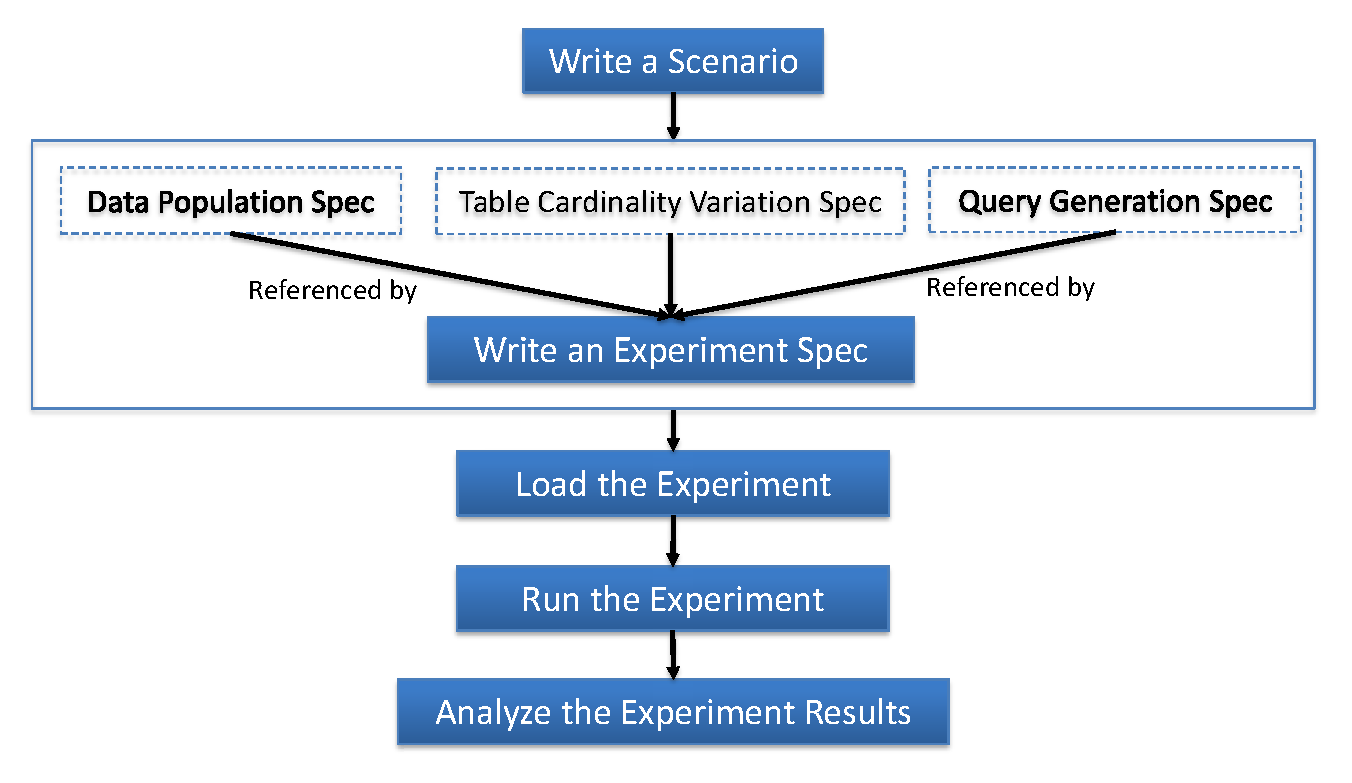
\includegraphics[scale=0.4]{./figures/exp_proc}
\caption{Experiment and analysis procedure~\label{fig:exp_proc}}
\end{figure}

\subsection{Experiment Specification}
Table~\ref{tab:exp_spec} exemplifies an experiment specification. 

\begin{table}[htp!]
\begin{center}
{
\scriptsize
\begin{tabular}{|p{8.5cm}|} \hline
\begin{minted}{xml}
<experiment name="op-1M-100q-1" scenario="onepass">
  <description>
    The baseline test of onepass scenario, with 100 
    predefined queries. Four experiment tables, 
    each with 1M rows. One variable table is used.
  </description>
  <dataDefinitionReference href="TestDataDef1M.xml"/>
  <tableConfiguration>
    <variableTableSet searchMethod="linear" 
    searchGranularity="10000">
      <table name="HT1" seed="1999">
        <cardinality hypotheticalMinimum="1"
         hypotheticalMaximum="2000000"/>
      </table>
    </variableTableSet>
    <fixedTableSet>
      <table name="HT2" seed="2999">
        <cardinality hypothetical="actual"/>
      </table>
      <table name="HT3" seed="3999">
        <cardinality hypothetical="actual"/>
      </table>
      <table name="HT4" seed="4999">
        <cardinality hypothetical="actual"/>
      </table>
    </fixedTableSet>
  </tableConfiguration>
   <queryDefinitionReference numberQueries="100" 
   type="predefinedQueries" href="100_q_1.xml"/>
</experiment>
\end{minted}
\\ \hline \end{tabular}
}
\caption{Example of an Experiment Specification~\label{tab:exp_spec}}
\end{center}
\end{table}

\paragraph{Data Definition}
Table~\ref{tab:data_spec} exemplifies an data population specification. 

\begin{table}[htp!]
\begin{center}
{
\scriptsize
\begin{tabular}{|p{8.5cm}|} \hline
\begin{minted}{xml}
<dataDefinition name="ft">
 <documentation>
 A database that has tables with cardinalities 
 that are a power of 10.  From 1 to 1,000,000.  
 There are only numeric column data in these tables.
 </documentation>
 <table name="HT1" cardinality="1000000">
  <column name="id1" dataType="number" dataLength="20" 
  dataGenerationType="sequential" distributionMinimum="0" 
  distributionMaximum="1000000" inPrimaryKey="true"/>
  ...
  <column name="id4" dataType="number" dataLength="20" 
  dataGenerationType="sequential" distributionMinimum="0" 
  distributionMaximum="1000000" inPrimaryKey="false"/>
 </table>
 ...
 <table name="HT4" cardinality="1000000">
 ...
 </table>
</dataDefinition>
\end{minted}
\\ \hline \end{tabular}
}
\caption{Example of a Data Population Specification~\label{tab:data_spec}}
\end{center}
\end{table}

\paragraph{Query Definition}
Table~\ref{tab:query_spec} exhibits an query generation specification. 

\begin{table}[htp!]
\begin{center}
{
\scriptsize
\begin{tabular}{|p{8.5cm}|} \hline
\begin{minted}{xml}
<queryDefinition numberQueries="100" 
javaClass="DefaultGrammarSpecificGenerator"
schemaFileName="/grammar.xsd">
    <grammar>
      <select maxColumns="4"/>
      <from maxNumCorrelationNames="4"/>
      <where cartesianPossible="false" maxPredicates="3">
        <binaryOperators>
          <operator symbol="="/>
        </binaryOperators>
        <binaryLogicalOperators>
          <operator symbol="AND"/>
        </binaryLogicalOperators>
        <unaryLogicalOperators>
          <operator symbol="NOT" usePercentage="0"/>
        </unaryLogicalOperators>
      </where>
      <aggregate function_name="SUM" percentage="50"/>
    </grammar>
  </queryDefinition>

\end{minted}
\\ \hline \end{tabular}
}
\caption{Example of an Query Generation Specification~\label{tab:query_spec}}
\end{center}
\end{table}

Table~\ref{tab:predefined_query_spec} shows a set of predefined queries. 

\begin{table}[htp!]
\begin{center}
{
\scriptsize
\begin{tabular}{|p{8.7cm}|} \hline
\begin{minted}{xml}
<predefinedQueries name = "100_q_1" >
<query sql="SELECT t3.id3, t3.id4, t0.id4, t3.id1 
FROM ft_HT4 t1, ft_HT1 t0, ft_HT3 t3, ft_HT2 t2  
WHERE (t1.id1=t0.id1 AND t0.id1=t3.id2 AND t3.id2=t2.id4)"/>
...
<query sql="SELECT t0.id2, SUM(t2.id4)  
FROM ft_HT1 t0, ft_HT2 t3, ft_HT1 t2, ft_HT1 t1  
WHERE (t0.id3=t3.id3 AND t3.id3=t2.id4 AND t2.id4=t1.id1) 
GROUP BY t0.id2"/>
</predefinedQueries>
\end{minted}
\\ \hline \end{tabular}
}
\caption{Example of a Pre-defined Query Specification~\label{tab:predefined_query_spec}}
\end{center}
\end{table}
  
\subsection{Experiment Run}
Experiment 
Figure~\ref{fig:exp_run_state} depicts the state change of an experiment run. 

\begin{figure}[htp!]
\centering
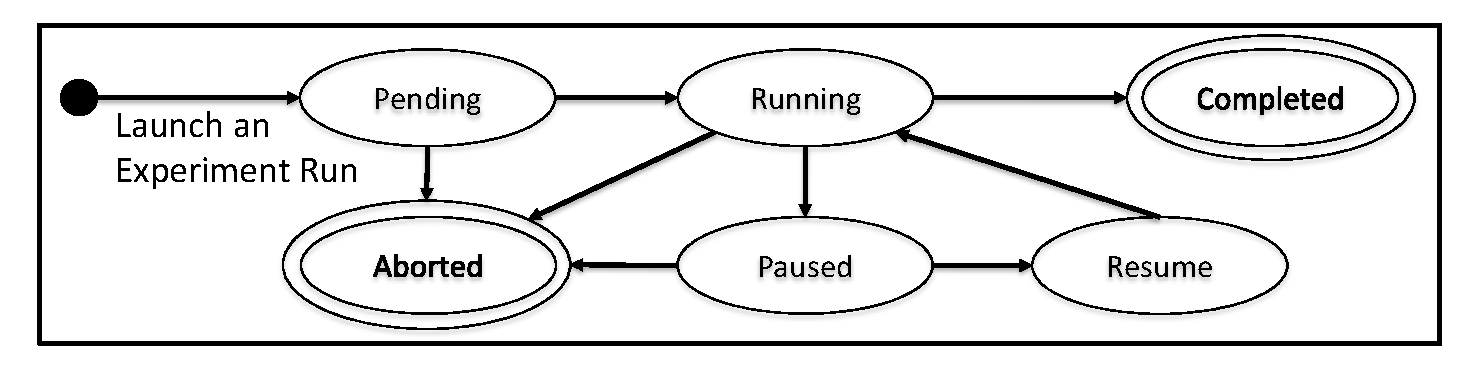
\includegraphics[scale=0.4]{./figures/exp_run_state}
\caption{Experiment run state diagram\label{fig:exp_run_state}}
\end{figure}
  
\section{Result Analysis}\label{sec:result_analysis}
Describe how Tucson protocol~\cite{Currim} is incorporated into {\sc AZDBLab}, 
and experiment results are passed to {\bf R} to do further analysis. 
The following items should be discussed in this section.

\begin{itemize}

\item Per-execution and per-process information extraction

\item (Discontinuity visualization)

\item Tucson protocol application (sanity check)
%is applied to refine our experiment results. The application procedure of the protocol are automatically 

\item Correlation analysis using R

\end{itemize}

\section{Related Work}\label{sec:related}
Provide a list of systems related to {\sc AZDBLab}.

\section{Summary and Future Work}\label{sec:summary}
Conclude this paper and talk about what needs to be done in future. 

\shorten{\section{Acknowledgments}
This research was supported in part by NSF grants\linebreak \hbox{IIS-0639106},
IIS-0415101, and EIA-0080123. We thank Ricardo Carlos, Preetha Chatterjee, Pallavi
Chilappagari, Jennifer Dempsey, David Gallup, Kevan Holdaway, Andrey
Kvochko, Siou Lin, Adam Robertson,
Lopamudra Sarangi, Linh Tran, Cheng Yi, and Man Zhang for
their contributions to the \hbox{\azdb} and Phil Kaslo, Tom Lowry, and John
Luiten for constructing and maintaining our experimental instrument\c2j{}{,
  a laboratory of six machines and associated software}.
}

%\vfill\pagebreak
%
% The following two commands are all you need in the
% initial runs of your .tex file to
% produce the bibliography for the citations in your paper.

% For peerreview papers, this IEEEtran command inserts a page break and
% creates the second title. It will be ignored for other modes.
\IEEEpeerreviewmaketitle

\bibliographystyle{./IEEEtran,./IEEEabrv}
\newcommand{\etalchar}[1]{$^{#1}$}
\begin{thebibliography}{99}

\vspace{0.1em}
\bibitem
{Currim}
S.~Currim, et. al., ``DBMS Metrology: Measuring Query Time'', in {\em Proceedings of the ACM SIGMOD conference},
pp.~261--272, 2013.
\bibitem
{Ram}
S. Ram and J. Liu, ``Understanding the Semantics of Data Provenance to Support Active 
Conceptual Modeling'', in {Proceedings of the International Workshop on Active Conceptual
Modeling of Learning}, P. P. Chen and Y. Wong (eds), LNCS 4512, Springer Verlag, 2007.
\bibitem
{Snodgrass99}
R. T. Snodgrass, ``Developing Time-Oriented Database Applications in SQL'', Morgan
Kaufmann Publishers, Inc., San Francisco, CA, July 1999, 504+xxiv pages
\end{thebibliography}
\end{document}
